

\chapter{Festlegung der Features}

Wie eingangs beschrieben handelt es sich um einen Feature basierten Algorithmus. Das hei\ss t, dass die
Merkmale eines Objekt im Bild, welches transformiert werden soll, zunächst erfasst werden müssen.
Beier und Neely nutzen dazu eine Liste aus gerichteten Linienpaaren: Einer Linie im Quellbild wird genau eine
Linie im Zielbild zugeordnet. Dabei werden die Linienpaare so platziert, sodass sie ein Merkmal
in den Bildern beschreiben. Zum Beispiel werden die Haaransätze der beiden Personen in Quell- und Zielbild
als Merkmale deklariert: Das Linienpaar wird dementsprechend gesetzt, siehe \ref{fig:linepairs}.

\begin{figure}[htbp]
	\centering
	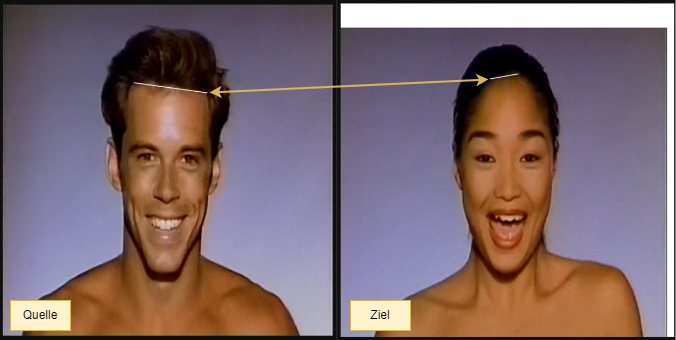
\includegraphics[width=0.9\textwidth]{linienpaare.drawio.png}
	\caption{Setzen eines Linienpaares}
	\label{fig:linepairs}
\end{figure}
Es ist wichtig zu beachten, dass die Linienpaare gerichtet sind. Die Linien besitzen also sowohl
Anfangs- als auch Endpunkt. Abbildung \ref{fig:linepairsfinal} zeigt die Linienpaare, welche für dass Resultat in
\ref{fig:morph} verantwortlich waren.
\begin{figure}[htbp]
	\centering
	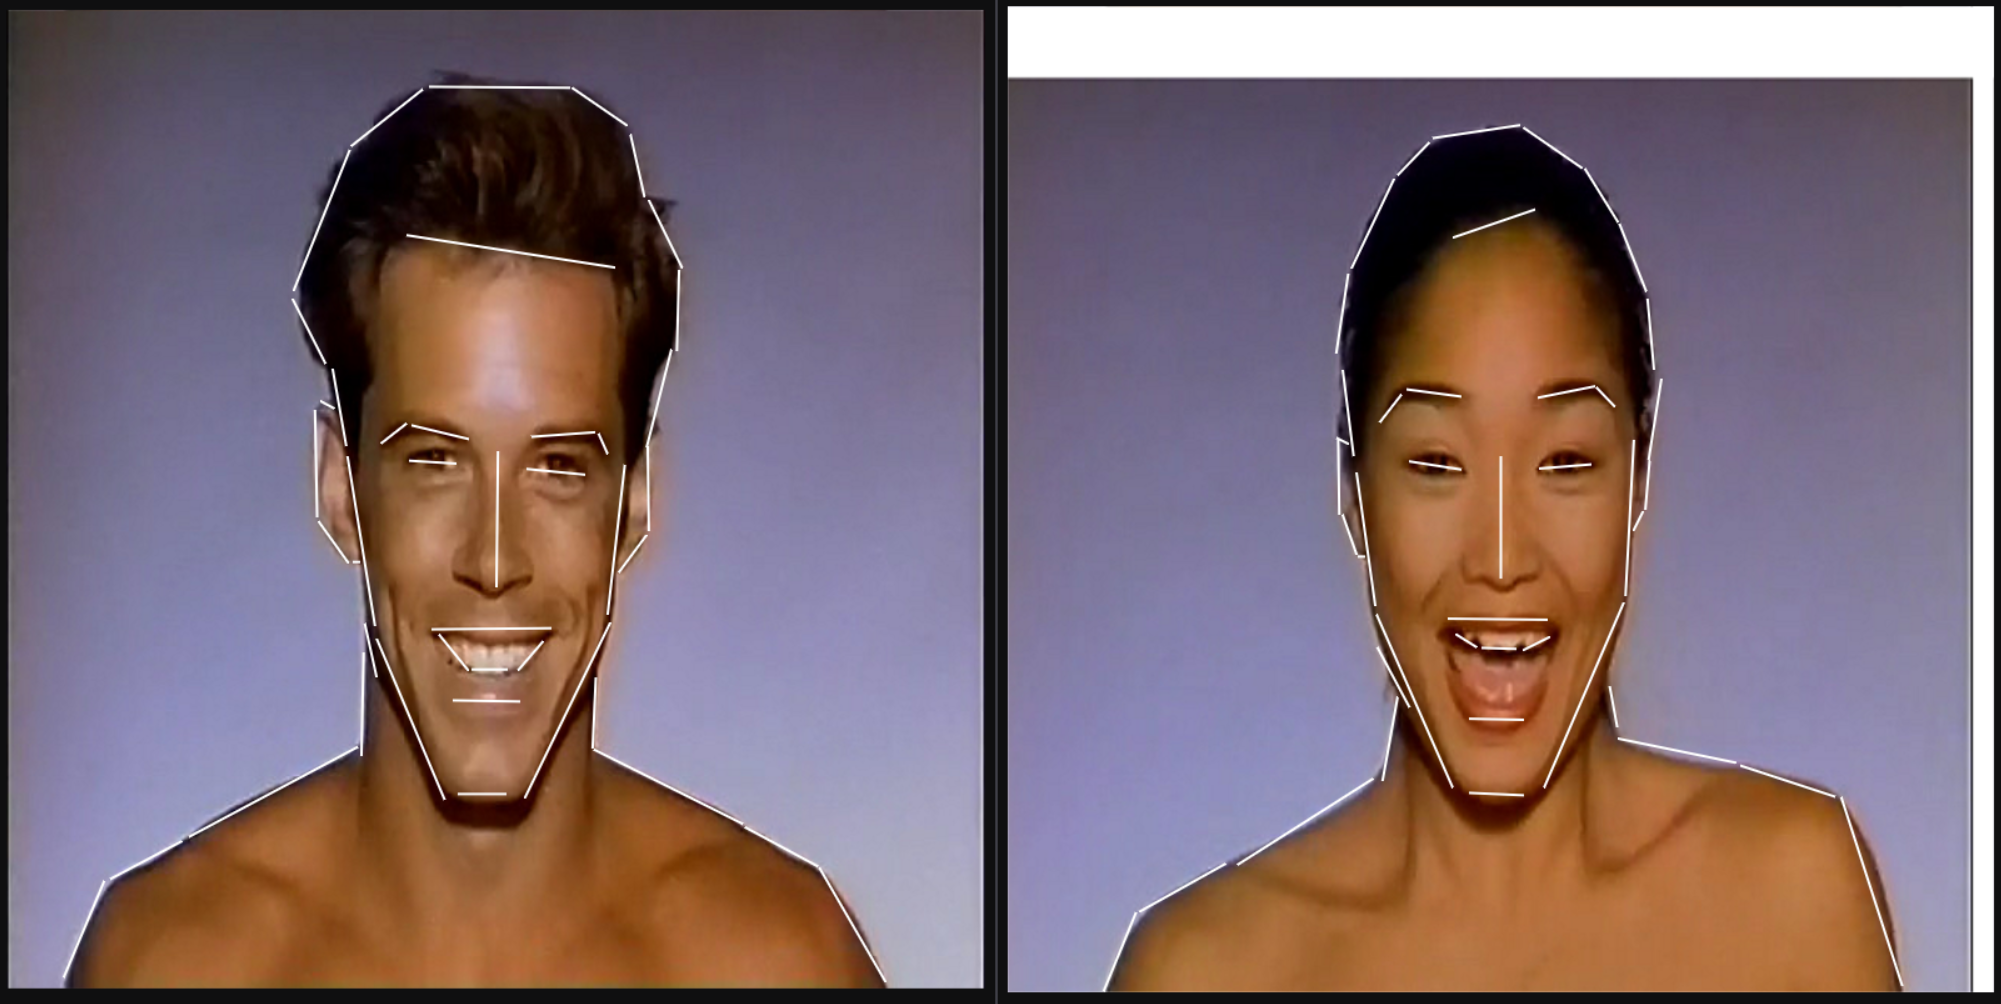
\includegraphics[width=0.9\textwidth]{linienpaarefinal.png}
	\caption{Finale Menge an Linienpaaren}
	\label{fig:linepairsfinal}
\end{figure}



